%!TEX root = ../thesis.tex
% створюємо розділ
\chapter{Оцінка стійкості реалізованої конструкції до вимог IND-CPA та IND-CCA}
\label{chap:chapter2}  

У цьому розділі буде здійснено аналіз відповідності реалізованої криптографічної конструкції вимогам двох основних моделей безпеки: IND-CPA та IND-CCA. Перш за все, розглянемо теоретичні основи цих моделей безпеки, щоб зрозуміти, як вони визначають рівень стійкості криптографічних схем. Далі буде проведена оцінка стійкості конструкції до цих вимог, а також порівняння стійкості конструкції до кожної з моделей. Завершальний етап включатиме практичну реалізацію атак, які дозволять перевірити, наскільки добре конструкція Baby Kyber витримує загрози згідно з обраними моделями безпеки.

%%% --------------------------------------------------------
\section{Вступ до моделей безпеки IND-CPA та IND-CCA}
%%% --------------------------------------------------------

\subsection*{IND-CPA стійкість}
 Безпека є найважливішою складовою будь-якої схеми і її забезпечення є головною задачею дослідника. Звичайне поняття безпеки дуже схоже на концепцію безпеки шифрування з відкритим ключем. Основною ідеєю є те, що зловмисник не повинен мати змогу визначити, чи міститься конкретний ключ в зашифрованому тексті. Інакше кажучи, зловмисник не повинен відрізнити випадковий ключ від ключа, який був зашифрований~\cite{KEMProof}. 

 Механізм інкапсуляції ключів вважається стійким до атаки обраним відкритим текстом (IND-CPA), якщо зловмисник $\mathcal{A}$ не може відрізнити спільний ключ від випадкового спільного ключа з імовірністю більше, ніж~$\frac{1}{2}$. Зловмисник $\mathcal{A}$ отримує всю відкриту інформацію, яка створена КЕМ. Це визначення параметризується розподілом S, який описує безпечне джерело спільних секретів. Варто зазначити, що КЕМ не має відкритого тексту, проте це поняття використовується у визначенні через аналогію з відповідними поняттями у шифруванні~\cite{Campagna2020}. 

Для доведення IND-CPA стійкості будують так звані IND-CPA ігри: 
\begin{figure}[h]
    \centering
    \renewcommand{\arraystretch}{1.5}
    \setlength{\tabcolsep}{6pt}
    
    \begin{tabular}{|c|}
        \hline
        \textbf{Game} $G0_{KEM}^{ind-cpa}(\mathcal{A})$ \\
        \hline
        $(\cdot, P) \gets_{\$} \textbf{KGen}()$ \\
        $(k, R) \gets_{\$} \textbf{Enc}(P)$ \\
        $\textbf{if } \perp(k, R) \textbf{ return } 0$ \\
        $\textbf{return } \mathcal{A}(P, R, k)$ \\
        \hline
    \end{tabular}
    \hspace{0.5cm}
    \begin{tabular}{|c|}
        \hline
        \textbf{Game} $G1_{KEM, S}^{ind-cpa}(\mathcal{A})$ \\
        \hline
        $(\cdot, P) \gets_{\$} \textbf{KGen}()$ \\
        $(k, R) \gets_{\$} \textbf{Enc}(P), k' \gets_{\$} \textbf{S}()$ \\
        $\textbf{if } \perp(k, R) \textbf{ return } 0$ \\
        $\textbf{return } \mathcal{A}(P, R, k')$ \\
        \hline
    \end{tabular}
    
    \caption{IND-CPA ігри}
\end{figure}

\begin{definition}~\cite{Campagna2020} (IND-CPA перевага)
    Нехай КЕМ --- механізм інкапсуляції ключів, $\mathcal{A}$ - алгоритм. Тоді, перевага $\mathcal{A}$ над IND-CPA KEM джерела S дорівнює: 
    $$Adv_{KEM, S}^{ind-cpa}(\mathcal{A}) = |Pr[G0_{KEM}^{ind-cpa}(\mathcal{A}) = 1] - Pr[G1_{KEM, S}^{ind-cpa}(\mathcal{A}) = 1] |$$
\end{definition}


\subsection*{IND-CCA стійкість}
 Існує і більш сильний варіант захисту. Тут зловмисник може робити запити на розшифрування вибраних ним зашифрованих текстів. Такі атаки називаються атаками на основі обраних шифротекстів (ССА). Вони моделюють ситуацію, у яких можливе знання ключів, що містяться в певних зашифрованих текстах. Хоча на практиці такі витоки зазвичай обмежені, більш загальна модель безпеки враховує ширший спектр загроз, що дозволяє побудувати схеми, які задовольняють загальну модель~\cite{KEMProof}. 

Насправді, концепція цієї атаки ідентична із IND-CPA за винятком того, що зловмисник також має змогу здійснити атаку за допомогою обраного шифротексту, адже має доступ до оракула декапсуляції. Він може викликати такий оракул для будь-яких шифротекстів, окрім тих які безпосередньо беруть участь у грі~\cite{Campagna2020}. 

Для доведення IND-CCA стійкості будують так звані IND-CCA ігри~\cite{Campagna2020}:
\begin{figure}[h]
    \centering
    \renewcommand{\arraystretch}{1.5}
    \setlength{\tabcolsep}{6pt}
    
    \begin{tabular}{|c|}
        \hline
        \textbf{Game} $G0^{ind-cca}_{KEM}(\mathcal{A})$ \\
        \hline
        $(sk, pk) \gets_{\$} \textbf{KGen}()$ \\
        $(k, c) \gets_{\$} \textbf{Enc}(pk)$ \\
        $\textbf{if } \perp(k) \textbf{ return } 0$ \\
        $\textbf{return } \mathcal{A}^{\mathcal{D}^{sk, c}}(pk, c, k)$ \\
        \hline
    \end{tabular}
    \hspace{0.5cm}
    \begin{tabular}{|c|}
        \hline
        \textbf{Game} $G1^{ind-cca}_{KEM, S}(\mathcal{A})$ \\
        \hline
        $(sk, pk) \gets_{\$} \textbf{KGen}()$ \\
        $(k, c) \gets_{\$} \textbf{Enc}(pk), k' \gets_{\$} \textbf{S}()$ \\
        $\textbf{if } \perp(k) \textbf{ return } 0$ \\
        $\textbf{return } \mathcal{A}^{\mathcal{D}^{sk, c}}(pk, c, k')$ \\
        \hline
    \end{tabular}
    
    \caption{IND-CCA games}
\end{figure}

\begin{definition}~\cite{Campagna2020} (IND-CСА перевага)
    Нехай КЕМ --- механізм інкапсуляції ключів, $\mathcal{A}$ - алгоритм зловмисника. Тоді, перевага $\mathcal{A}$ над IND-CCA KEM джерела S дорівнює: 
    $$Adv_{KEM, S}^{ind-cca}(\mathcal{A}) = |Pr[G0_{KEM}^{ind-cca}(\mathcal{A}) = 1] - Pr[G1_{KEM, S}^{ind-cca}(\mathcal{A}) = 1] |$$
\end{definition}


%%% --------------------------------------------------------
\section{Оцінка стійкості Baby Kyber до вимог IND-CPA та IND~-CCA}
%%% --------------------------------------------------------

\subsection*{Оцінка стійкості Baby Kyber до IND-CPA}

Стійкість криптографічної схеми до атаки IND-CPA є одним із важливих критеріїв її безпеки. Для оцінки цієї стійкості необхідно проаналізувати здатність зловмисника відрізнити зашифровані версії двох різних повідомлень, згенерованих за допомогою відкритого ключа, без доступу до особистого ключа. У контексті Baby Kyber, ця стійкість визначається здатністю схемі забезпечити безпечне шифрування, яке не дозволяє зловмиснику здобути корисну інформацію про повідомлення, навіть якщо він має доступ до численних зашифрованих повідомлень.

Для доведення стійкості побудуємо IND-CPA гру. Гра IND-CPA моделює атаку зловмисника, який має доступ до відкритого ключа та оракула шифрування. Мета --- перевірити, чи зможе він відрізнити, яке з двох повідомлень було зашифроване.

\textbf{1. Ініціалізація}

Оракул генерує ключі для Baby Kyber:
\begin{itemize}
    \item Випадкова матриця: $A \in \mathbb{Z}_q[X]^{k \times k} / (X^n + 1)$.
    \item Вектори $s, e \sim \text{CBD}$ --- шум, згенерований через центральний біноміальний розподіл.
    \item Обчислення: $t = A s + e$.
    \item Відкритий ключ: $pk = (A, t)$, особистий ключ: $sk = s$.
    \item Оракул передає зловмиснику $pk$.
\end{itemize}

\textbf{2. Шифрування}

Зловмисник $\mathcal{A}$ може багаторазово шифрувати повідомлення $m$:
\begin{enumerate}
    \item Надсилає $m$ до оракула.
    \item Оракул:
    \begin{itemize}
        \item Вибирає $r, e_1, e_2 \sim \text{CBD}$.
        \item Обчислює шифротекст:
        \[
        u = A^T r + e_1,\quad v = t^T r + e_2 + \left\lfloor \frac{q}{2} \right\rfloor m.
        \]
        \item Повертає $c = (u, v)$.
    \end{itemize}
\end{enumerate}

\textbf{3. Вибір повідомлень (Challenge Phase)}

\begin{itemize}
    \item Супротивник обирає два повідомлення $m_0, m_1$ однакової довжини.
    \item Надсилає $(m_0, m_1)$ оракулу.
    \item Оракул вибирає випадковий біт $b \in \{0, 1\}$ та нові випадкові $r^*, e_1^*, e_2^*$.
    \item Обчислює:
    \[
    u^* = A^T r^* + e_1^*,\quad v^* = t^T r^* + e_2^* + \left\lfloor \frac{q}{2} \right\rfloor m_b.
    \]
    \item Повертає $c^* = (u^*, v^*)$ супротивнику.
\end{itemize}

\textbf{4. Вгадування}

\begin{itemize}
    \item Супротивник аналізує $c^*$ та видає здогад $b' \in \{0, 1\}$.
    \item Якщо $b' = b$, то супротивник виграв гру.
\end{itemize}


\begin{figure}[h]
    \centering
    \renewcommand{\arraystretch}{1.5}
    \setlength{\tabcolsep}{6pt}
    
    \begin{tabular}{|c|}
        \hline
        \textbf{Game} $G_0^{\mathsf{ind\text{-}cpa}}(\mathcal{A})$ \\
        \hline
        $(s, e) \gets_{\$} \text{CBD}$ \\
        $A \gets_{\$} \mathbb{Z}_q[X]^{k \times k} / (X^n + 1)$ \\
        $t = A s + e$ \\
        $pk = (A, t),\quad sk = s$ \\
        $\mathcal{A}$ receives $pk$ and access to $\mathsf{Enc}(\cdot)$ \\
        $(m_0, m_1) \gets \mathcal{A}$ \\
        $b \gets_{\$} \{0,1\}$ \\
        $r, e_1, e_2 \gets_{\$} \text{CBD}$ \\
        $u = A^T r + e_1$ \\
        $v = t^T r + e_2 + \left\lfloor \frac{q}{2} \right\rfloor m_b$ \\
        $c^* = (u, v)$ \\
        $b' \gets \mathcal{A}(c^*)$ \\
        \textbf{return} $[b' = b]$ \\
        \hline
    \end{tabular}
    
    \caption{IND-CPA гра для Baby Kyber}
\end{figure}

\newpage
Щоб з'ясувати, чи може зловмисник визначити біт $b$, розглянемо, наскільки компоненти шифротексту $u$ та $v$ приховують інформацію про повідомлення $m_b$.

\textbf{Розподіл $u$}

Шифротекст $u$ визначається як:
\[
u = A^T r + e_1
\]
\begin{itemize}
    \item $A$ --- публічна випадкова матриця поліномів.
    \item $r \sim \text{CBD}$ --- випадковий вектор поліномів, незалежний від $A$.
    \item  $A^T r$ --- виглядає як випадковий вектор.
    \item Додавання шуму $e_1$ (також з розподілу CBD) ще більше ускладнює структуру $u$.
\end{itemize}

$u$ виглядає як повністю випадковий вектор, незалежний від $m_b$.

\textbf{Розподіл $v$}

Компонент $v$ задається як:
\[
v = t^T r + e_2 + \left\lfloor \frac{q}{2} \right\rfloor m_b
\]
Підставимо $t = A s + e$:
\[
\begin{aligned}
v &= (A s + e)^T r + e_2 + \left\lfloor \frac{q}{2} \right\rfloor m_b \\
  &= s^T (A^T r) + e^T r + e_2 + \left\lfloor \frac{q}{2} \right\rfloor m_b
\end{aligned}
\]

\begin{itemize}
    \item $s$ --- секретний вектор, недоступний для супротивника.
    \item $A^T r$ --- випадковий вектор, незалежний від $s$.
    \item Добуток $s^T (A^T r)$ має вигляд випадкового полінома.
    \item Шум $e^T r + e_2$ ще більше маскує значення.
\end{itemize}

$v$ також виглядає як випадковий елемент, і $m_b$ у ньому не видимий через шум.


IND-CPA-стійкість означає, що зловмисник не може відрізнити, яке з двох повідомлень $m_0, m_1$ було зашифроване, навіть маючи доступ до:
\begin{itemize}
    \item Публічного ключа $pk = (A, t)$.
    \item Оракула шифрування: $\mathsf{Encrypt}(pk, \cdot)$.
    \item Шифротексту $c^* = (u, v)$, що містить зашифроване $m_b$.
\end{itemize}

Схема є IND-CPA стійкою тому що: 
\begin{itemize}
    \item Рандомізація через $r$ гарантує, що одне й те саме повідомлення шифрується кожного разу інакше.
    \item Шумові доданки $e_1$, $e_2$ та $e$ приховують структуру повідомлення.
    \item Без знання $s$ неможливо відновити $m_b$ з $v$.
    \item Побудовано на задачі Learning With Errors (LWE), яка вважається складною навіть для квантових обчислень.
\end{itemize}

Інформація про $m_b$ не витікає із шифротексту, тому схема є стійкою до IND-CPA атак.


\subsection*{Оцінка стійкості Baby Kyber до IND-CCA}

Стійкість криптографічної схеми до атаки IND-CCA є більш суворим критерієм безпеки, ніж стійкість до IND-CPA. У цьому випадку зловмисник може не лише отримати зашифровані повідомлення, а й зробити запити на дешифрування обраних шифротекстів, що дає йому додаткову інформацію, яку можна використати для атаки на схему. Оцінка стійкості Baby Kyber до IND-CCA ґрунтується на здатності схеми зберігати конфіденційність повідомлення навіть при наявності такого доступу до шифротекстів.

Для доведення стійкості побудуємо IND-CСA гру. Гра IND-CСA моделює атаку зловмисника, який має доступ до відкритого ключа, оракула шифрування та оракула дешифрування. Мета --- перевірити, чи зможе він відрізнити, яке з двох повідомлень було зашифроване.

\textbf{1. Ініціалізація}

Оракул генерує ключі для Baby Kyber:

– Випадкова матриця:  
\[
A \in \mathbb{Z}_q[X]^{k \times k} / (X^n + 1)
\]

– Вектори $s, e \sim \text{CBD}$ — шум, згенерований через центрований біноміальний розподіл.

– Обчислення:
\[
t = As + e
\]

– Відкритий ключ: $pk = (A, t)$, особистий ключ: $sk = s$.

– Оракул передає зловмиснику $pk$.

– Також зловмиснику надається доступ до оракула дешифрування: $\mathcal{D}(c) = \mathsf{Dec}_{sk}(c)$, з обмеженням, що не можна подавати $c = c^*$ у фазі виклику.

\textbf{2. Шифрування}

Зловмисник $\mathcal{A}$ може багаторазово шифрувати повідомлення $m$:

1) Надсилає $m$ до оракула.

2) Оракул:

– Вибирає $r, e_1, e_2 \sim \text{CBD}$.

– Обчислює шифротекст:
\[
u = A^T r + e_1, \quad v = t^T r + e_2 + \left\lfloor \frac{q}{2} \right\rfloor m
\]

– Повертає $c = (u, v)$.

– Зловмисник може також надсилати запити на дешифрування довільних $c \ne c^*$, використовуючи оракул $\mathcal{D}$.

\textbf{3. Вибір повідомлень (Challenge Phase)}

– Зловмисник обирає два повідомлення $m_0, m_1$ однакової довжини.

– Надсилає $(m_0, m_1)$ оракулу.

– Оракул вибирає випадковий біт $b \in \{0,1\}$ та нові випадкові значення $r^*, e_1^*, e_2^*$.

– Обчислює:
\[
u^* = A^T r^* + e_1^*, \quad v^* = t^T r^* + e_2^* + \left\lfloor \frac{q}{2} \right\rfloor m_b
\]

– Повертає $c^* = (u^*, v^*)$ зловмиснику.

– Забороняє надсилати $c^*$ до оракула дешифрування.

\textbf{4. Вгадування}

– Зловмисник аналізує $c^*$, продовжує робити дозволені запити до оракула дешифрування $\mathcal{D}(c \ne c^*)$.

– Видає здогад $b' \in \{0, 1\}$.

– Якщо $b' = b$, то зловмисник виграв гру.


\begin{figure}[h]
    \centering
    \renewcommand{\arraystretch}{1.6}
    \setlength{\tabcolsep}{8pt}

    \begin{tabular}{|p{7.1cm}|p{6.7cm}|}
        \hline
        \multicolumn{2}{|c|}{\textbf{Game} $G_0^{\mathsf{ind\text{-}cca}}(\mathcal{A})$} \\
        \hline
        $(s, e) \gets_{\$} \text{CBD}$ & $A \gets_{\$} \mathbb{Z}_q[X]^{k \times k} / (X^n + 1)$ \\
        $t = As + e$ & $pk = (A, t),\quad sk = s$ \\
        \textit{$\mathcal{A}$ receives $pk$, access to $\mathsf{Enc}(\cdot)$ and $\mathsf{Dec}(\cdot \ne c^*)$} & \\
        $(m_0, m_1) \gets \mathcal{A},\quad b \gets_{\$} \{0,1\}$ & \\
        $r^*, e_1^*, e_2^* \gets_{\$} \text{CBD}$ & $u^* = A^T r^* + e_1^*$ \\
        $v^* = t^T r^* + e_2^* + \left\lfloor \frac{q}{2} \right\rfloor m_b$ & $c^* = (u^*, v^*)$ \\
        \textit{$\mathcal{A}$ may query $\mathsf{Dec}(c)$ for $c \ne c^*$} & \\
        $b' \gets \mathcal{A}(c^*)$ & \\
        \multicolumn{2}{|c|}{\textbf{return} $[b' = b]$} \\
        \hline
    \end{tabular}

    \caption{IND-CCA гра для Baby Kyber}
\end{figure}


Щоб з’ясувати, чи може зловмисник визначити біт $b$, розглянемо, наскільки компоненти шифротексту $u$ та $v$ приховують інформацію про повідомлення $m_b$, якщо зловмисник має доступ до оракула дешифрування.

\textbf{Модель атаки}

У моделі IND-CCA зловмисник має доступ до:

\begin{itemize}
    \item Публічного ключа $pk = (A, t)$
    \item Оракула шифрування: $\mathsf{Enc}(pk, \cdot)$
    \item Оракула дешифрування: $\mathsf{Dec}(sk, \cdot)$, з обмеженням $c \ne c^*$
\end{itemize}

Задача зловмисника — вгадати біт $b$ за шифротекстом $c^* = (u^*, v^*)$, який є шифруванням одного з повідомлень $m_0, m_1$.

\textbf{Вразливість шифротексту}

Challenge-шифротекст має вигляд:
\[
c^* = (u^*, v^*) = (A^T r^* + e_1^*,\quad t^T r^* + e_2^* + \left\lfloor \frac{q}{2} \right\rfloor m_b)
\]

Супротивник може сконструювати змінений шифротекст:
\[
c' = (u^*, v^* + \delta)
\]
і передати його на дешифрування. Якщо $m_b = 1$, $v^*$ має зсув $\left\lfloor \frac{q}{2} \right\rfloor$, якщо $m_b = 0$ — ні.

Проаналізувавши результат розшифрування $c'$, зловмисник може зробити висновок про значення $m_b$.

\textbf{Відсутність цілісності}

Схема Baby Kyber не містить механізму перевірки автентичності:

\begin{itemize}
    \item Немає хеш-функцій або автентифікаторів у шифротексті
    \item Немає симетричної перевірки чи зв’язування $u$ і $v$
    \item Шум $e_1$, $e_2$ не гарантує безпеку від модифікації
\end{itemize}

Це дозволяє зловмиснику модифікувати $v^*$ та отримувати детерміновану зміну результату дешифрування.

Отже, зловмисник може розшифрувати змінений шифротекст $c'$ на основі $c^*$. А результат дешифрування допомагає вивести біт $b$. Саме тому схема не є IND-CCA стійкою.



\subsection*{Порівняння стійкості до IND-CPA та IND-CCA}

\begin{table}[h]
    \centering
    \renewcommand{\arraystretch}{1.6}
    \setlength{\tabcolsep}{10pt}
    \caption{Порівняння стійкості Baby Kyber до IND-CPA та IND-CCA}
    \begin{tabular}{|p{5.3cm}|p{4.5cm}|p{4.5cm}|}
        \hline
        \textbf{Критерій} & \textbf{IND-CPA} & \textbf{IND-CCA} \\
        \hline
        Модель зловмисника & Має доступ до шифрування (Enc), може надсилати будь-які повідомлення & Має доступ до шифрування (Enc) і дешифрування (Dec), крім $c^*$ \\
        \hline
        Доступ до дешифрування & Відсутній & Дозволено, але $c \ne c^*$ \\
        \hline
        Тип атаки & Вибір відкритого тексту (Chosen Plaintext) & Вибір шифротексту (Chosen Ciphertext) \\
        \hline
        Стійкість Baby Kyber & Стійкий & Не стійкий \\
        \hline
        Причини стійкості / нестійкості & Випадковість $r$, шум $e_1, e_2$ та структура $v$ приховують $m_b$ & Можна модифікувати $v^*$ і проаналізувати відповідь дешифрування \\
        \hline
        Приховування $m_b$ & Ефективне через шум і LWE & Частково порушується через можливість змінювати $v$ \\
        \hline
        Перевірка цілісності шифротексту &  Відсутня, але не критично &  Відсутня, що робить можливими атаки \\
        \hline
        Основна уразливість & — & Challenge можна змінити, зловмисник аналізує результат \\
        \hline
        Захист від модифікації $c^*$ & — &  Відсутній \\
        \hline
        Рівень безпеки & Семантична безпека при шифруванні & Семантична безпека + автентичність \\
        \hline
    \end{tabular}
\end{table}

Проведене порівняння показує, що Baby Kyber є надійною схемою шифрування з відкритим ключем у моделі IND-CPA, але не забезпечує захисту від IND-CCA атак.

У моделі IND-CPA зловмисник обмежений лише доступом до шифрування. У такому середовищі Baby Kyber демонструє високу стійкість завдяки використанню:
\begin{itemize}
    \item випадкових векторів при шифруванні;
    \item шумових членів, що маскують повідомлення;
    \item математичної складності задачі Learning With Errors (LWE).
\end{itemize}

Однак у моделі IND-CCA, де зловмисник також має доступ до оракула дешифрування, виявляється серйозна вразливість. Через відсутність перевірки цілісності шифротексту, зловмисник може модифікувати частину challenge-шифротексту (наприклад, компонент $v^*$) і використовувати оракул дешифрування для витоку інформації про зашифроване повідомлення. Це робить Baby Kyber нестійким до IND-CCA атак у базовій формі.


%%% --------------------------------------------------------
\section{Практична реалізація атак на відповідність моделям IND-CPA та IND-CCA}
%%% --------------------------------------------------------

У цьому підрозділі буде розглянуто практичну реалізацію атак IND-CPA та IND-CCA на спрощену версію Baby Kyber.  Буде подано опис основних компонентів атак, включаючи побудову викликів з боку супротивника, моделювання доступу до оракула шифрування та аналіз виграшу. Завершальною частиною стане перевірка коректності реалізації та оцінка ймовірності успішної атаки відповідно до теоретичних моделей IND-CPA та IND-CCA, описаних вище.

\subsection*{Реалізація атаки для IND-CPA}

З метою оцінки стійкості реалізованої спрощеної версії Baby Kyber до IND-CPA-атак, було проведено експеримент, в якому моделюється поведінка зловмисника з доступом до оракула шифрування.

Для реалізації атаки було створено адаптивну стратегію, за якою зловмисник:

\begin{enumerate}
    \item Ініціалізує параметри криптосистеми: розмір кільця $n$, модуль $q$, параметри шуму $\eta$ тощо, та генерує відкритий ключ $(A, t)$ і особистий ключ~$s$.
    
    \item Обирає два повідомлення $m_0$ і $m_1$, які представлені векторами з нулів та одиниць відповідно.
    
    \item Отримує шифротексти для обох повідомлень — $c_0$ та $c_1$, — та обчислює їхні оцінки, що ґрунтуються на сумі перших коефіцієнтів шифротекстів $u[0][0]$ та $v[0]$.
    
    \item Отримує шифротекст виклику $c^\star$ на одному з повідомлень $m_b$, де біт $b$ обирається випадковим чином.
    
    \item Порівнює оцінку $c^\star$ з оцінками $c_0$ та $c_1$ та вгадує, яке з повідомлень було зашифровано. Якщо відстань до $c_0$ менша — зловмисник вгадує $b=0$, інакше — $b=1$.
    
    \item Підраховує кількість успішних вгадувань за велику кількість запусків та оцінює статистичну значущість результатів.
\end{enumerate}

Результати експерименту виводяться у вигляді:
\begin{itemize}
    \item Кількості вдалих вгадувань правильного повідомлення;
    \item Ймовірності успішного вгадування;
    \item Виграшу зловмисника порівняно з випадковим вгадуванням;
    \item p-значення (p-value), що вказує на статистичну значущість результатів;
    \item 95\% довірчого інтервалу.
\end{itemize}

Для перевірки гіпотези про те, що зловмисник діє не краще за випадкове вгадування, було використано біноміальний тест із пакету \texttt{scipy.stats}. Статистичний аналіз дозволяє зробити висновки про вразливість реалізації до IND-CPA атак.

\textbf{Результати тестування:} нижче детально описані результати атаки, зображені на рисунку~\ref{fig:ind_cpa_1}.

\begin{itemize}
    \item Adversary success rate = 4971/10000
    \item Probability of guessing correctly =  $0.4971$: значення $0.4971$ для ймовірності успішного вгадування майже дорівнює $0.5$ — як випадкове вгадування.
    \item Advantage over random guessing = $0.0029$: перевага над випадковим вгадуванням advantage становить лише $0.0029$, тобто дуже мала.
    \item p-value (binomial test) =  $0.5687$: p-value більше за $0.05$, а отже ми не можемо відхилити нульову гіпотезу про те, що результат досягнутий випадково.
    \item 95\% confidence interval $[0.4873,\ 0.5069]$ : довірчий інтервал містить значення $0.5$, що підтверджує: статистично результат не є підозрілим.
\end{itemize}

Результати виконання атаки зображені на наступних рисунках : 

\begin{figure}[h]
    \centering
    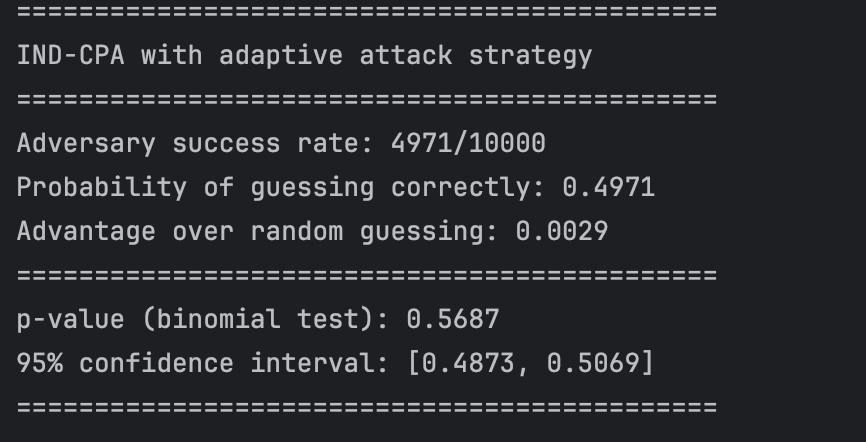
\includegraphics[width=0.925\textwidth]{ПРАКТИКА/Images/IND_CPA_1.jpg}
    \caption{Результат атаки 1}
    \label{fig:ind_cpa_1}
\end{figure}

\begin{figure}[h]
    \centering
    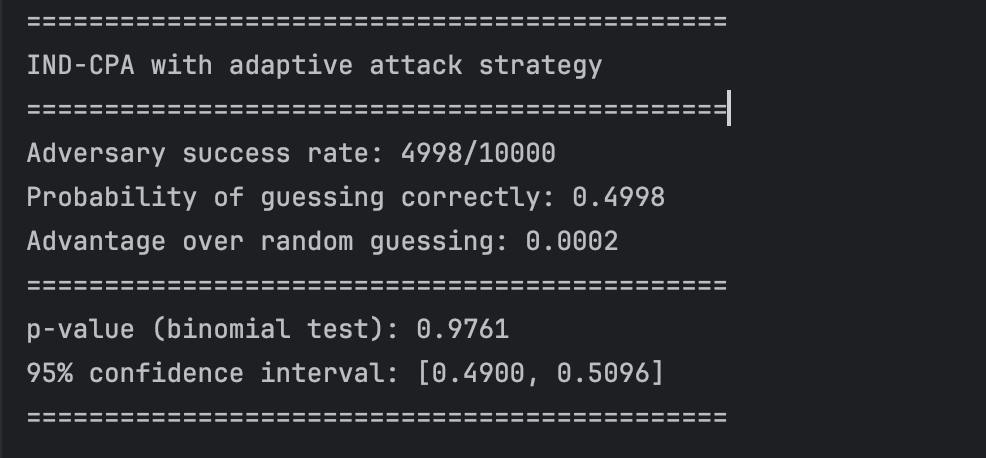
\includegraphics[width=0.925\textwidth]{ПРАКТИКА/Images/IND_CPA_2.jpg}
    \caption{Результат атаки 2}
    \label{fig:ind_cpa_2}
\end{figure}

На основі наведених результатів можна зробити висновок, що реалізований алгоритм Baby Kyber пройшов тест на стійкість до IND-CPA атаки. Успішність атакувальника статистично не відрізняється від випадкового вгадування, отже, шифрування є стійким у цій моделі безпеки.

\subsection*{Реалізація атаки для IND-CCA}

Для оцінки стійкості реалізованої версії Baby Kyber до IND-CCA - атаки було реалізовано експеримент, який моделює зловмисника, що має обмежений доступ до оракула розшифрування — без можливості розшифровувати виклик (challenge ciphertext) $c^\star$.

Атака ґрунтується на модифікації виклику $c^\star$ та аналізі результату розшифрування модифікованого шифротексту. Загальна стратегія виглядає так:

\begin{enumerate}
    \item Ініціалізується схема Baby Kyber з параметрами $q$, $n$, $k$, $\eta$. Генеруються ключі: матриця $A$, вектор $t$ та секретний ключ $s$.

    \item Зловмисник обирає два повідомлення $m_0 = [0, 0, \dots, 0]$ та $m_1 = [1, 1, \dots, 1]$, та отримує шифротекст $c^\star$ для одного з них ($m_b$), де біт $b$ обирається випадково.

    \item Створюється оракул розшифрування $D(\cdot)$, який відмовляється обробляти запити на $c^\star$, але дозволяє всі інші.

    \item Зловмисник модифікує компоненту $v^\star$ шифротексту $c^\star$, додаючи до неї невеликий відомий зсув, отримуючи змінений шифротекст $c'$.

    \item Модифікований шифротекст $c'$ передається до оракула $D(\cdot)$, який повертає розшифроване повідомлення.

    \item Якщо сума елементів у результаті розшифрування ближча до $[1, 1, \dots, 1]$, то зловмисник вгадує, що було зашифровано $m_1$, інакше — $m_0$.

    \item Після $N$ повторень експерименту обчислюються статистичні показники атаки.
\end{enumerate}

Оцінка результатів включає:

\begin{itemize}
    \item Загальну кількість вдалих вгадувань бітів $b$.
    \item Імовірність правильного вгадування ($\hat{p}$).
    \item Виграш зловмисника відносно випадкового вгадування ($|\hat{p} - 0.5|$).
    \item p-значення біноміального тесту, що оцінює статистичну значущість результату.
    \item 95\% довірчий інтервал для $\hat{p}$.
\end{itemize}

Атака демонструє можливість відхилення від ідеальної IND-CCA стійкості за рахунок експлуатації навіть мінімальних змін у шифротексті. 

\textbf{Результати тестування:} нижче детально описані результати атаки, зображені на рисунку~\ref{fig:ind_cca_1}.

\begin{itemize}
    \item Adversary success rate = 10000/10000
    \item Probability of guessing correctly = $1.0000$: ймовірність успішного вгадування становить 100\%, що свідчить про повну успішність атаки.
    \item Advantage over random guessing = $0.5000$: перевага над випадковим вгадуванням є максимальною — атакувальник завжди визначає правильне повідомлення.
    \item p-value (binomial test) = $0.0000$: надзвичайно низьке значення p-value означає, що ймовірність досягнення такого результату випадково практично нульова.
    \item 95\% confidence interval $[1.0000,\ 1.0000]$: довірчий інтервал повністю охоплює значення $1.0$, що підтверджує абсолютну впевненість у результаті.
\end{itemize}

На основі наведених результатів можна зробити висновок, що реалізований алгоритм Baby Kyber не є стійким до IND-CCA атаки. Атакувальник мав повну можливість відрізнити зашифровані повідомлення, що свідчить про критичну уразливість у цій моделі безпеки. Для забезпечення повної криптографічної стійкості необхідно впровадити відповідні механізми захисту від атак із вибраним шифротекстом.

\newpage
Результати виконання атаки зображені на рисунку:

\begin{figure}[h]
    \centering
    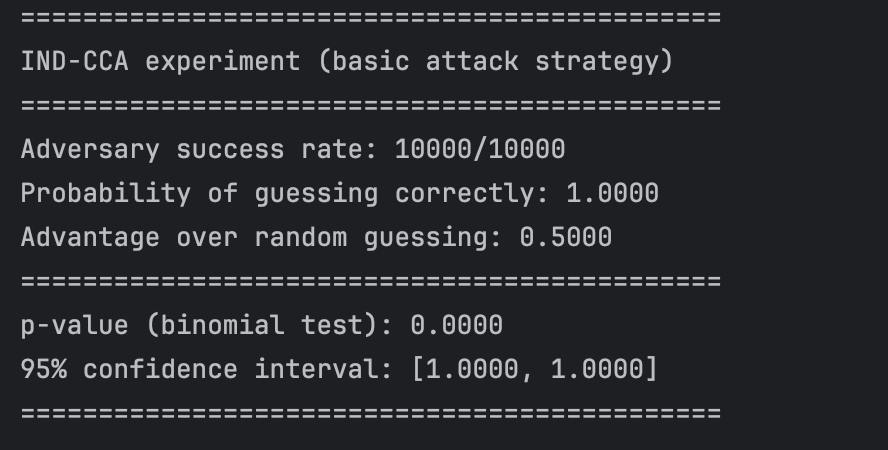
\includegraphics[width=0.925\textwidth]{ПРАКТИКА/Images/IND_CCA_1.jpg}
    \caption{Результат атаки}
    \label{fig:ind_cca_1}
\end{figure}


